\documentclass[12pt]{article}
\usepackage{amssymb, amsmath}
\usepackage{bm}
\usepackage{dsfont}
\usepackage{empheq}
\usepackage{graphicx}
\usepackage{float}

% Set up the margins.
\usepackage[top=1in, bottom=1in, left=1in, right=1in]{geometry}

\begin{document}



\title{Data Science Take-Home-Assignment Report}

\author{William Wong}
\date{October 11, 2017}

\maketitle


\section{Detection of Stops}

\subsection{The Kalman Filter}
To detect when a user stops, I primarily use a Kalman filter to track his/her position along with the velocity in two dimensions. The (hidden) internal state $X(t)$ evolves according to
\begin{equation}
  X(t+1) = F X(t) + W(t) \, ,
\end{equation}
where $X(t)$ contains the two dimensional longitude and latitude, along with the velocities
\begin{equation}
X(t) = \begin{bmatrix}
    x_1(t) \\
    x_2(t) \\
    v_1(t) \\
    v_2(t)
    \end{bmatrix} \, .
\end{equation}
$F$ is the forward-transition model
\begin{equation}
F = \begin{bmatrix}
    1 & 0 & \Delta t & 0 \\
    0 & 1 & 0 & \Delta t \\
    0 & 0 & 1 & 0 \\
    0 & 0 & 0 & 1
    \end{bmatrix} \, ,
\end{equation}
and $W(t) \sim \mathcal{N}(0, Q(t))$.

The observation at time $t$ is $Y(t)$
\begin{equation}
  Y(t) = H X(t) + V(t) \, ,
\end{equation}
where $V(t) \sim \mathcal{N}(0, R(t))$.

We use the {\tt pykalman} library in Python to implement the Kalman filter.
We consider a user has stopped when the absolute value of the estimated rates of change are both less than some parameter.

Sample results obtained from the Kalman filter are shown in Fig.~\ref{fig:kalman01}, where the following quantities are plotted as a function of time:
\begin{enumerate}
  \item raw latitude data and the estimated latitude.
  \item the estimated rate of change of latitude.
  \item raw longitude data and the estimated longitude.
  \item the estimated rate of change of longitude.
  \item whether the user has stopped.
\end{enumerate}

\begin{figure}[H]
\centering
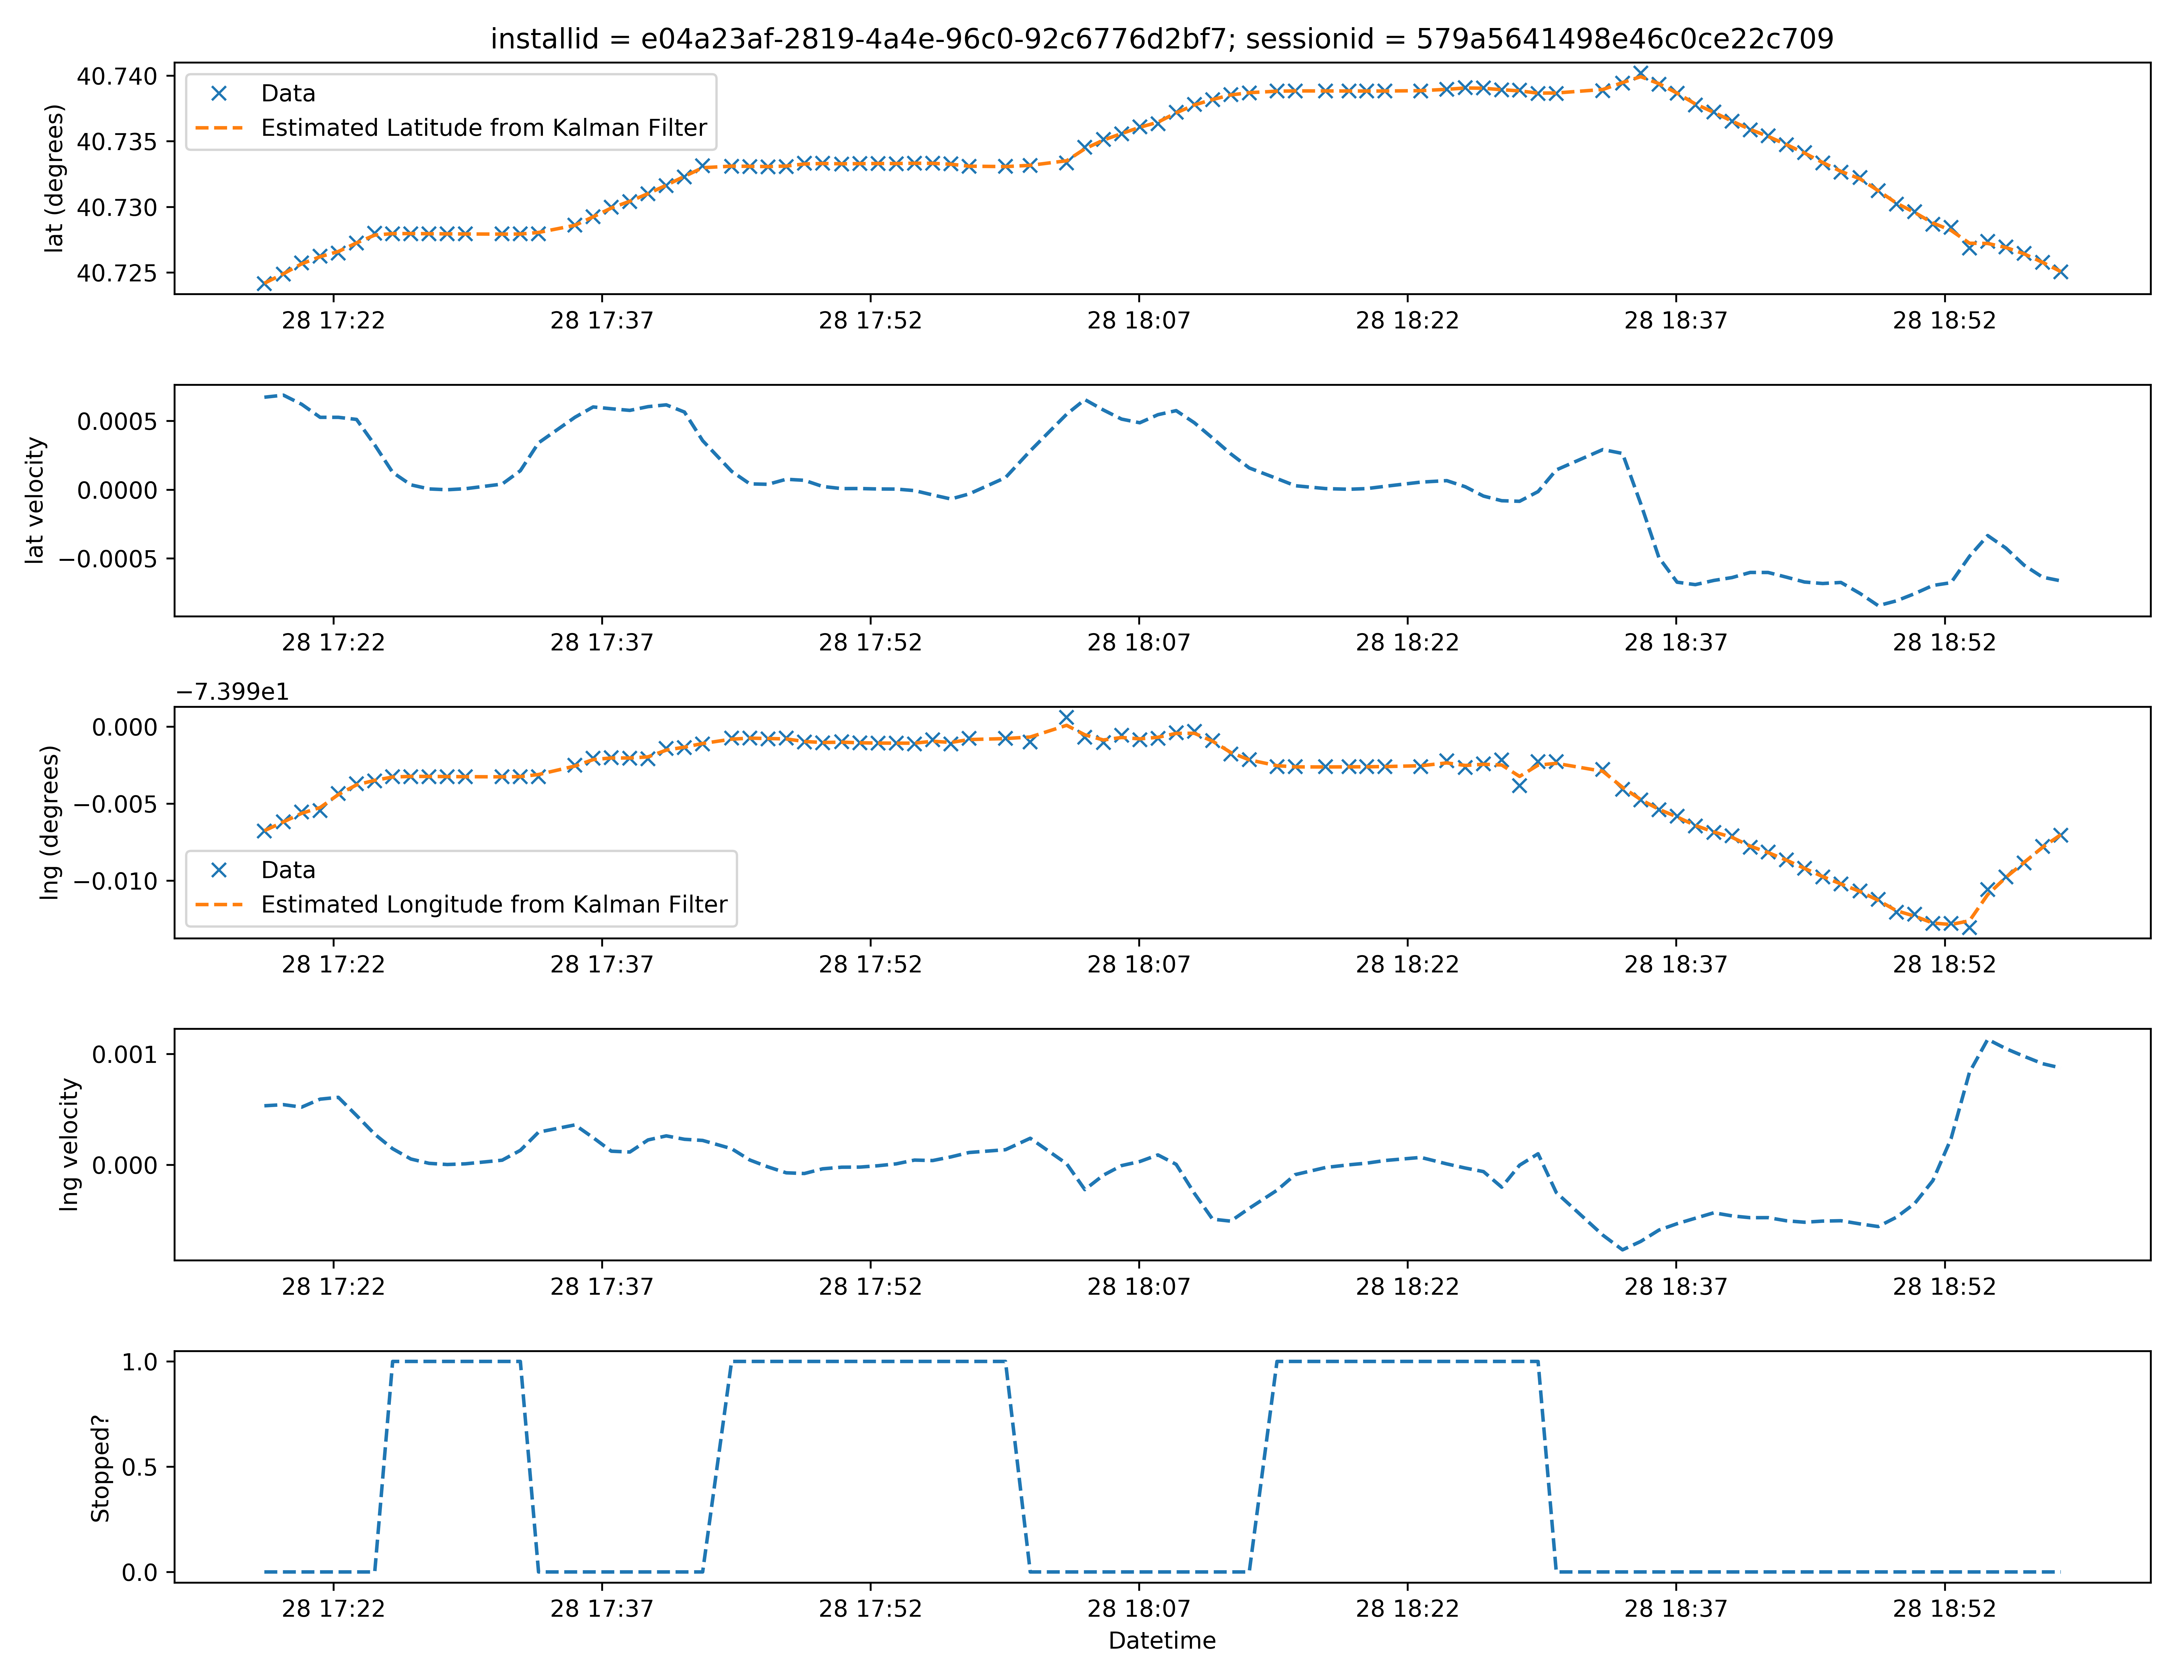
\includegraphics[width=6.5in]{graphics/kalman01.png}
\caption{Sample results obtained from the Kalman filter.}
\label{fig:kalman01}
\end{figure}


\subsection{The DBSCAN Algorithm}
We also applied the DBSCAN algorithm in Python to estimate the clusters when users stop.  I use the haversine metric and the ball-tree algorithm to calculate great-circle distances between points.
Sample results obtained from using the DBSCAN algorithm are shown in Fig.~\ref{fig:dbscan01}

\begin{figure}[H]
\centering
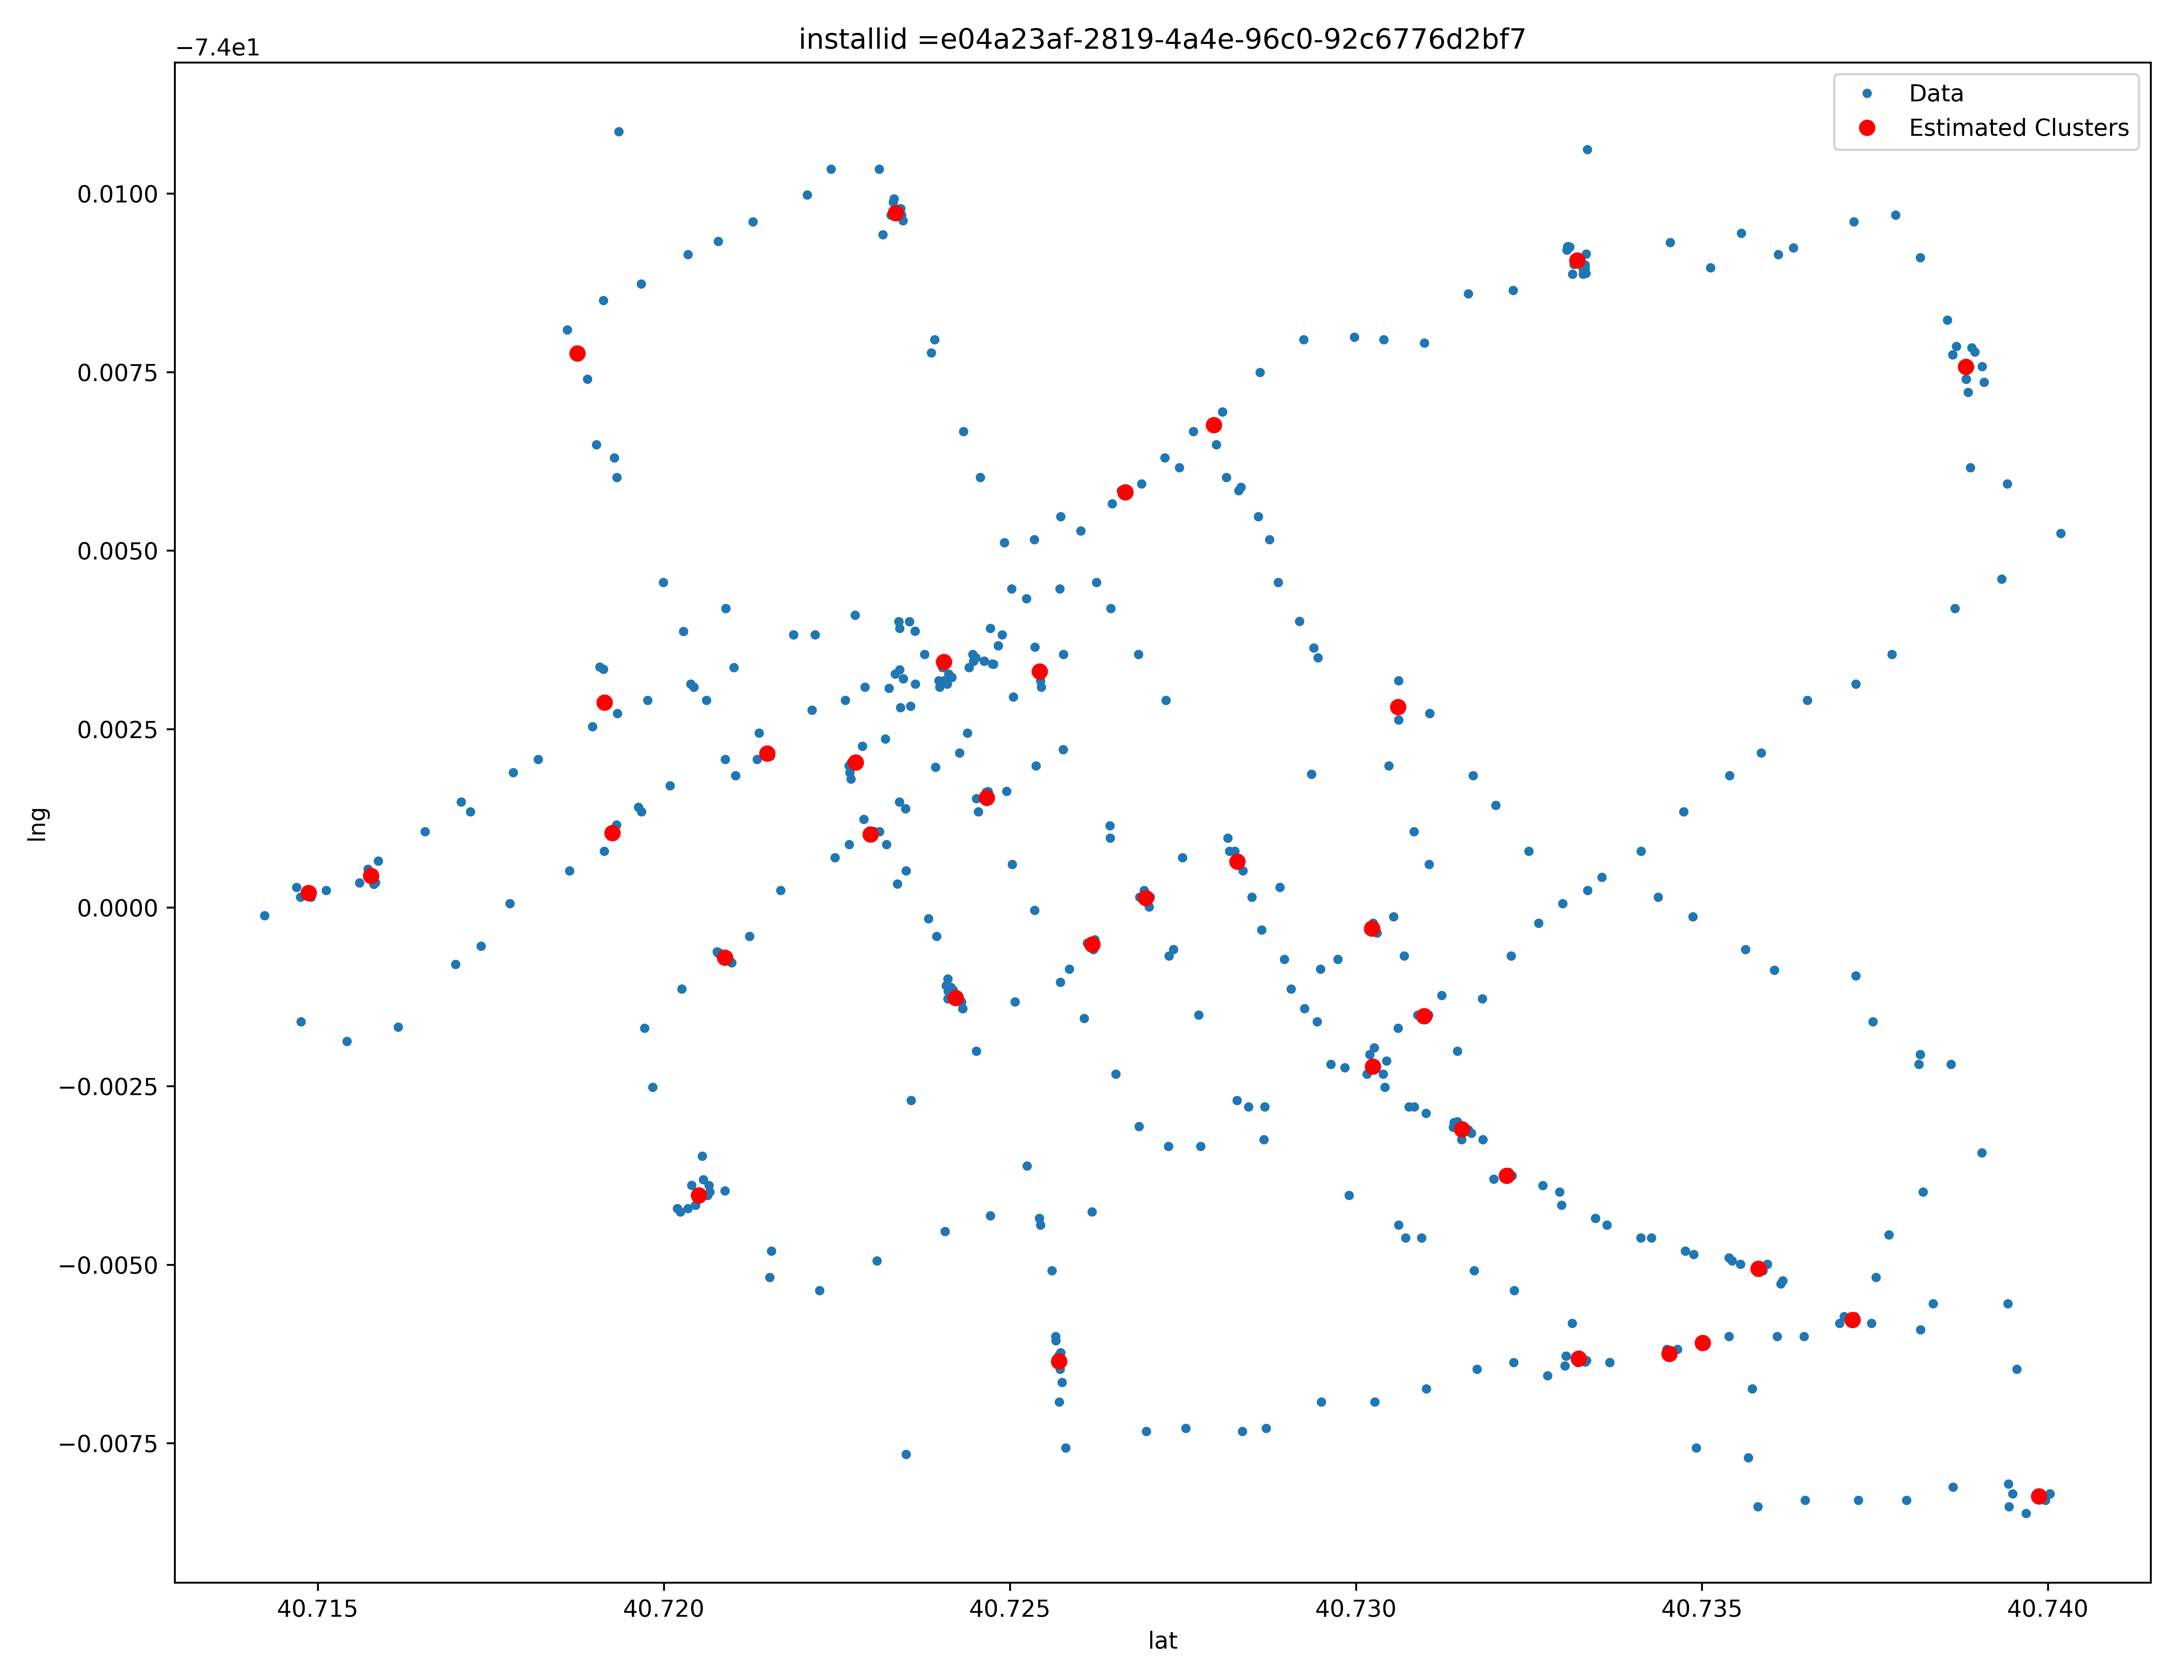
\includegraphics[width=6.5in]{graphics/dbscan01.png}
\caption{Sample results obtained from using the DBSCAN algorithm.}
\label{fig:dbscan01}
\end{figure}

\end{document}

